\chapter{Introduction and Motivation}\label{ch:intro}

Lung cancer is the most common cancer in the world in men, both in amount of cases and mortality. In women, is third in cases and second in mortality, after breast cancer\cite{WCR2014}. Yearly deaths due to lung cancer go over 1.5 million (see figure \ref{fig:world} for incidence), having around 10\% of five year survival rate in developed countries, and much lower in developing countries\cite{CRUK2014}. One over fourteen people has a lifetime risk of developing lung cancer\cite{Harrisons2012}, in average between men and women. The high incidence and mortality rates has lead to a big amount of research in research fields from all disciplines, in order to push further the detection and treatment of the disease, with an output of over 23.000 lung cancer related research articles in prestigious journals in the last 10 years\cite{Nature2015}. In addition, the  actual lung cancer treatment has been transformed from non-existent in the 70s to used worldwide\cite{Comis2003}.


\begin{figure}[ht]
\begin{center}
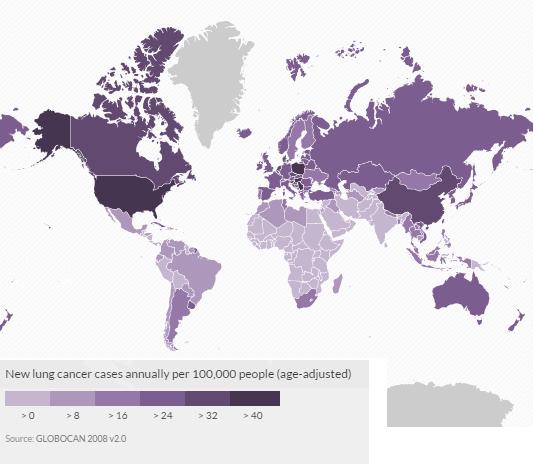
\includegraphics[width=0.98\columnwidth]{StateOfArt/worldmap.png}
\caption[Lung cancer incidence in the world]{Lung cancer incidence per country, age adjusted data. Map and data from {GLOBOCAN}\cite{GLOBOCAN2010}.}
%IARC has proprietary rights to the materials on the Website. Publications/data made available by IARC/WHO enjoy copyright protection in accordance with the provisions of Protocol 2 of the Universal Copyright Convention. All rights are reserved. Materials (fact sheets, maps, estimates or data) may be used "as is" for research, educational or other non-commercial purposes, but the corresponding reference must be cited in all cases.
\label{fig:world}
\end{center}
\end{figure}



The treatment of lung cancer varies between different types, but there are four main techniques: Chemotherapy, lobectomy or pneumoctomy, radiotherapy (RT) and palliative care. Generally, in early stages of small cell lung cancer the typical treatment would consist in chemotherapy with radiotherapy, and then brain radiotherapy, as there is chance that the tumour would spread to the head when treated. If the tumour has been detected in a very early stage and has not spread to the lymph nodes a lobectomy may be performed, removing part of the lung. Usually this is followed by radiotherapy and chemotherapy to make sure the tumour is killed.
In the case of non-small cell lung cancer, in the first stages a lobectomy or a pneumoctomy (removal of the whole lung) may be performed. Generally radiotherapy and chemotherapy (less likely) are also performed. In the last stages of the cancer, usually the treatment is palliative care i.e. treatments to reduce the symptoms and relief pain\cite{CRUK2014b}.

In practically all stages of different lung cancer treatments, radiotherapy is extensively used as above half of the treated patients do undergo the procedure\cite{Cancerorg}. About 120.000 patients use radiotherapy in the UK every year. Radiotherapy aims to kill malignant cells using ionizing radiation, generally using photons. High energy photons (X-rays) ionize the atoms that are part of the DNA chain. In photon therapy, this happens due to the ionization of the water in the cells, that forms free radicals, such as hydroxyl radicals, destroying the DNA of the cells and killing them.

Conventional photon RT is widely used around the world, nowadays generally guided by imaging systems during treatment planning (image guided radiation therapy, IGRT). Imaging systems, such as computed tomography (CT) and magnetic resonance imaging (MRI) are used to carefully tune the X-ray beam to focus in the specific location and shape of the tumour, and monitor the effects during the whole treatment period. However, a different type of radiation therapy exists, particle therapy or hardron therapy, that uses charged particles instead of photons, by accelerating them with circular particle accelerators. These particles (protons and heavy ions)  penetrate the tissue with minimal interaction and release almost all the energy before stopping. Figure \ref{fig:bragg} shows the energy deposition (Dose) plotted versus the penetration of the energy beam in tissue. The energy burst that hardron show is refereed as the Bragg peak, after its discoverer William Henry Bragg. The Bragg peak allows for a radiation therapy where a larger amount of healthy tissue can be spared, while delivering highly spatially accurate doses to only the tumour areas. While the growth of hardron therapy has been slow in the past due to its cost, it is not being accelerated thanks to international collaboration projects such as ENLIGHT\cite{dosanjhparticle}, with 100 centres estimated by 2020 around the globe, 30 of them in Europe, 3 of them being already on their final stages in construction in the UK.

\begin{figure}[ht]
\begin{center}
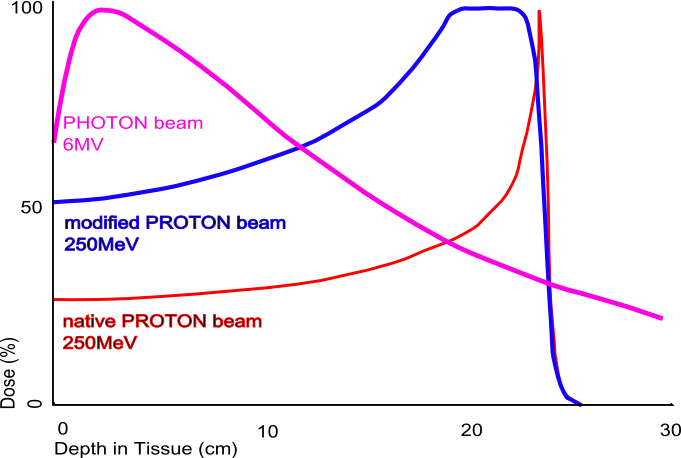
\includegraphics[width=0.6\columnwidth]{Introduction/BraggPeak.png}
\caption[Bragg peak]{The dose produced by a native and by a modified proton beam in passing through tissue, compared to the absorption of a photon or x-ray beam.\cite{bragg}}
%GNU license, wikipedia
\label{fig:bragg}
\end{center}
\end{figure}


As previously mentioned, for both types of RT but specially for hadron therapy, imaging is generally used and needed for accurate treatment. Tumours not only are very different between patients, but also change considerably during treatment, so the patient does due to the physical toll of cancer treatment. This means that the tumour does change both shape and location, and that if these changes are not known, healthy tissue could be damaged and cancerous tissue spared. Generally patients will be imaged before each treatment, being one of the most common systems for imaging cone beam compute tomography (CBCT). CBCT takes few hundreds of seconds to scan a patient due to mechanical safety limitations. As one can foresee, this is an important limiting factor for tumour that move, such the liver and the lung ones, as the motion during acquisition can generate heave artefacts around the moving parts in image reconstruction. This moving effect is also a key factor to take into account in hadron therapy, as having a moving tumour means the high chance of missing the treatment target. Providing accurate imaging not only in space, but in time (4D imaging) is a key factor on treatment planning, an thus in cancer treatment. This thesis is about that.


% Iterative algorithms

% GPU computing



\section{Aim of the thesis}
%  Talk about: 
\section{Thesis organization}


